\documentclass[xcolor=dvipsnames,mathserif,9pt]{beamer} %handout
%\usefonttheme{serif}%{structurebold}%{structuresmallcapsserif}%{serif}

\usepackage{graphicx}
\usepackage{amsmath}
\usepackage{amssymb}
\usepackage[font=footnotesize]{caption} % set the captain font size to 8 (i.e. footnotesize)
\usepackage{subfig} % uses subfloats within a single float MUST after the package {caption}!!
\usepackage{natbib}
%\usepackage{cite} % sort the reference in the article by number or alphabatic
\usepackage{color}
\usepackage{algorithm} % options: boxed [section]
\usepackage{algpseudocode} % for algorithm
%\usepackage{enumerate}
\usepackage{enumitem} % directly use itemize, easily specify indent and everything
\setlist[itemize]{leftmargin=*,label=$\bullet$}%leftmargin=*,itemsep=0pt} %topsep=5pt
\setlist[enumerate]{label={\arabic*)}}
\usepackage{hyperref}
\usepackage{wrapfig}
\usepackage{textpos}
\usepackage{bibentry} % for publication list
\makeatletter\let\saved@bibitem\@bibitem\makeatother % make hyperref and bibentry compatible!!!
\nobibliography*
\usepackage{fancybox}% shadow for image
%\usepackage{empheq} % emphasize equations
\usepackage{bm}
\usepackage{arydshln} % for dashline in table or matrix
\linespread{1.3}
\usepackage{multimedia}

\usepackage{setspace} \setstretch{1.2}

\usepackage{framed}
\colorlet{shadecolor}{black!5}
% for box, page breakable, very good!!
\usepackage[framemethod=TikZ]{mdframed}%
\mdfdefinestyle{myFrame}{%
    linecolor=gray!15!white,%gray
    outerlinewidth=0.1pt,
    roundcorner=3pt,
    skipabove=15pt, % the space before the entire box
    skipbelow=15pt, % the space after the entire box. Please see the figure 2 in the manual, very clear!
    innertopmargin=10pt,%\baselineskip,
    innerbottommargin=10pt,%\baselineskip,
    %innerrightmargin=10pt,
    %innerleftmargin=10pt,
    splittopskip=\baselineskip,
    splitbottomskip=\baselineskip,
    backgroundcolor=gray!10!white,
    frametitlerule=true,
    frametitlebackgroundcolor=gray!20!white,
    frametitleaboveskip=5pt,
    frametitlebelowskip=5pt,
}
\mdfdefinestyle{myAlgo}{%
    linecolor=gray!100!white,%gray
    outerlinewidth=0.1pt,
    roundcorner=3pt,
    skipabove=15pt, % the space before the entire box
    skipbelow=15pt, % the space after the entire box. Please see the figure 2 in the manual, very clear!
    innertopmargin=10pt,%\baselineskip,
    innerbottommargin=10pt,%\baselineskip,
    %innerrightmargin=10pt,
    %innerleftmargin=10pt,
    splittopskip=\baselineskip,
    splitbottomskip=\baselineskip,
    backgroundcolor=gray!0!white,
    frametitlerule=true,
    frametitlebackgroundcolor=gray!20!white,
    frametitleaboveskip=5pt,
    frametitlebelowskip=5pt,
}


\usepackage{tikz}
\usetikzlibrary{calc} % for calculation functions in Tikz let, in commands in Tikz
\usetikzlibrary{shapes} % for block diagram
\usetikzlibrary{chains}
\usetikzlibrary{fit}
\usetikzlibrary{arrows}
\usetikzlibrary{decorations.text} % text along path

\newcommand{\blue}[1]{\textcolor{blue}{#1}}
\definecolor{myred}{RGB}{200,0,0}
\newcommand{\red}[1]{\textcolor{myred}{#1}} %magenta purple
\newcommand{\I}{\mathcal{I}}
\newcommand{\tr}{\mathrm{tr}}
\newcommand{\Null}{\mathrm{Null}}
\newcommand{\Range}{\mathrm{Range}}
\newcommand{\one}{\mathbf{1}}
\newcommand{\rank}{\mathrm{rank}}
\newcommand{\myspan}{\mathrm{span}}
\newcommand{\mydiag}{\mathrm{diag}}
\newcommand{\D}{\mathrm{d}}
\renewcommand{\d}{\mathrm{d}}
\newcommand{\blkdiag}{\mathrm{blkdiag}}
\newcommand{\sgn}{\mathrm{sgn}}
\newcommand{\T}{\mathrm{T}}
\newcommand{\myqed}{\hfill$\blacksquare$}
\newcommand{\ep}{\varepsilon}
\newcommand{\sig}{\mathrm{sig}_a}
%\newcommand{\sigep_}[1]{\sig(\ep_{#1})}
\newcommand{\R}{\mathbb{R}}
\newcommand{\A}{\mathcal{A}}
\newcommand{\G}{\mathcal{G}}
\newcommand{\E}{\mathbb{E}}
\newcommand{\X}{\mathcal{X}}
\newcommand{\V}{\mathcal{V}}
\newcommand{\N}{\mathcal{N}}
\newcommand{\M}{\mathcal{M}}
\renewcommand{\H}{\mathcal{H}}
\renewcommand{\L}{\mathcal{B}}
\renewcommand{\S}{\mathcal{S}}
\newcommand{\xe}{x_{\text{e}}}
%\newcommand{\Null}[1]{\mathrm{Null}\left(#1\right)}
\newcommand{\sk}[1]{\left[#1\right]_\times} % skew symmetric operator
\newcommand{\dia}[1]{\mathrm{diag}\left(#1\right)} % block diagnal matrix
%\renewcommand{\span}[1]{\mathrm{span}\left\{#1\right\}} % ERROR when redefine \span
\newcommand{\Var}{\mathrm{Var}}
\newcommand{\var}{\mathrm{var}}


\graphicspath{{figures/}}

% for tikz, theorem, lemma ... environments have already been declared. You don't need to declare, or you need to use other names than theorem or lemma, such as my_theorem.
%\newtheorem{my_theorem}{Theorem}
%\newtheorem{my_lemma}{Lemma}
\newtheorem{assumption}{Assumption} % necessary for beamer
%\newtheorem{my_remark}{Remark}
\newtheorem{proposition}{Proposition} % necessary for beamer
%\newtheorem{my_corollary}{Corollary}
%\newtheorem{my_example}{Example}
%\newtheorem{my_definition}{Definition}
%\newtheorem{my_problem}{Problem}

%##################################################
\newcommand{\pagetitle}[1]{\textbf{\textcolor{BlueViolet}{$\circ$ #1}}} %!!!
\newcommand{\pagehighlight}[1]{\textbf{\textcolor{Brown}{#1}}} %!!!
\newcommand{\mypause}{\pause} % this is useful for slide show. if you don't want pause any more, just set it as blank
%\newcommand{\mybullet}{\textcolor{BlueViolet}{$\blacksquare$} }%{$\rhd$ }
%\newcommand{\myhighsign}{$\star$ }% the sign to highlight a sentence

%##################################################
% To highlight equation. Example: \begin{align*} \boxed{xxx} \end{align*}
% does not support multiline equations
% put color to \boxed math command
\newcommand*{\boxcolor}{gray}
\makeatletter
\renewcommand{\boxed}[1]{\textcolor{\boxcolor}{%
%\tikz[baseline={([yshift=-1ex]current bounding box.center)}] \node [rectangle, minimum width=1ex,rounded corners,draw] {\normalcolor\m@th$\displaystyle#1$};}}
\tikz[baseline={([yshift=-1ex]current bounding box.center)}] \node [rectangle, minimum width=2ex,rounded corners,draw] {\normalcolor\m@th$\displaystyle#1$};}}
\makeatother

%##################################################
% set my own theme
\def\structureHeight{9mm}
\usetheme[height=\structureHeight]{Rochester}
\usecolortheme[RGB={0,0,128}]{structure}
\setbeamertemplate{items}[circle]%rectangle, triangle,circle
\setbeamertemplate{blocks}[rounded][shadow=true]
\setbeamertemplate{navigation symbols}{}
%\addtobeamertemplate{frametitle}{} % specify the logo
%{
%    \begin{textblock*}{100mm}(.87\textwidth,-\structureHeight)
%        \includegraphics[height=6.6mm,width=3cm,keepaspectratio]{../common_figures_private/westlake_logo.png} % add logo
%    \end{textblock*}
%}
\addtobeamertemplate{frametitle}{\vskip4pt}{} % specify
%\setbeamerfont{frametitle}{size=\large}
\definecolor{mylightgray}{RGB}{240 240 240}
\definecolor{mykhaki}{RGB}{240 230 140}% khaki color
\definecolor{mylightYellow}{RGB}{255,255,224} % light yellow
%\setbeamercolor{beamercolor1}{bg=mylightgray, fg=black}
%\setbeamercolor{beamercolor2}{bg=mylightYellow,fg=black}%{bg=yellow!90!white, fg=black}
% background and foreground color
\setbeamercolor{background canvas}{bg=black!0!white} % background color of every slide! My previous value was black!10!white for my lecture videos!
\setbeamercolor{normal text}{bg=black!10!white} % background color for e.g. theorem environment. When canvas is 10, here it can be 20; the bg for normal text changes the color of hidden text when you use overlay

\setbeamercolor{block title}{bg=mykhaki,fg=black}
\defbeamertemplate{footline}{zsy_frameNumber}
{%
  \hspace{5pt}  \emph{Shiyu Zhao}
  \hspace*{\fill}%
  \usebeamercolor[fg]{page number in head/foot}%
  \insertframenumber\,/\,\inserttotalframenumber \vspace{0pt} \hspace{5pt}
  \vskip5pt
}
\setbeamertemplate{footline}[zsy_frameNumber]
%##################################################
\setbeamercovered{transparent=0} % a good value for transparent text is 20
% when using the overlay commands like \onslide or \uncover, the text will NOT be invisible, instead it will be like transparent
%\pause will also have the transparent effect: command \pause is easy to use: to make it invisible, change the value to zero.



\usepackage{multimedia}

\newcommand{\hl}{$\triangleright$ }
%\newcommand{\blue}[1]{\textcolor{blue}{#1}}
%\newcommand{\red}[1]{\textcolor{red}{#1}}
%\newcommand{\I}{\mathcal{I}}
\begin{document}

%%%%%%%%%%%%%%%%%%%%%%%%%%%%%%%%%%%%%%%%%%%%%%%%%%%%%%%%%%%%%%%%%%%%%%%%%%%%%%%%%
% define the author, date etc. information
%\subtitle{Mathematical and Biological Foundation for Reinforcement Learning}
\title{Lecture 2: State Value and Bellman Equation}

\author{Shiyu Zhao
\newline
\newline {\small Department of Artificial Intelligence}
\newline {\small Westlake University}
}
%\logo{\includegraphics[width=1cm,height=1cm,keepaspectratio]{NUSLogo.png}~}
%\date{\today}
\date{}
\subject{}


%%%%%%%%%%%%%%%%%%%%%%%%%%%%%%%%%%%%%%%%%%%%%%%%%%%%%%%%%%%%%%%%%%%%%%%%%%%%%%%%%

{
\setbeamertemplate{footline}{} % remove the frame number of the title page
\begin{frame}
    %\frametitle{Lecture: Networked Dynamic Systems}
    \addtocounter{framenumber}{-1} % discounter the title page, otherwise the frame number starts from 2 instead of 1
    \titlepage % this only gives the author etc. information
\end{frame}
}


\begin{frame}
\frametitle{Outline}
\begin{figure}[h]
  \centering
\includegraphics[width=0.8\linewidth]{Figure_chapterRelationship.pdf}
\end{figure}
\end{frame}


\begin{frame}
\frametitle{Introduction}

\begin{itemize}
\item In the last lecture, we introduced Monte-Carlo learning.

\item In the next lecture, we will introduce temporal-difference (TD) learning.

\item In this lecture, we press the pause button to get us better prepared.

Why?

\pause

\begin{itemize}
\item[-] There is a \blue{knowledge gap}!
\item[-] The ideas and expressions of TD algorithms are \blue{very different} from the algorithms we studied so far.
\item[-] Many students who see the TD algorithms the first time many wonder why these algorithms were designed in the first place and why they work effectively.
\end{itemize}

\end{itemize}

\end{frame}
%---------------------
\begin{frame}
\frametitle{Introduction}

In this lecture,
\begin{itemize}
\item We fill the knowledge gap between the previous and upcoming lectures by introducing basic \blue{stochastic approximation (SA)}  algorithms.
\item We will see in the next lecture that the \blue{temporal-difference algorithms are special SA algorithms}. As a result, it will be much easier to understand these algorithms.
\item We will also study the important algorithm of \blue{stochastic gradient descent (SGD)}.
\end{itemize}

\end{frame}
%---------------------
\begin{frame}
\frametitle{Outline}
\tableofcontents
\end{frame}
\AtBeginSection[]% put it to the start of each section
{
  \begin{frame}
    \frametitle{Outline}
    \tableofcontents[currentsection]
  \end{frame}
}
%--------------------------------------
\AtBeginSection[]% put it to the start of each section
{
  \begin{frame}
    \frametitle{Outline}
    \tableofcontents[currentsection]
  \end{frame}
}
\section{Motivating examples}
%---------------------
\begin{frame}
\frametitle{Motivating example: mean estimation, again}
\textbf{\blue{Revisit} the mean estimation problem:}
\begin{itemize}
\item Consider a random variable $X$.
\pause
\item Suppose that we collected a sequence of iid samples $\{x_i\}_{i=1}^N$.
\pause
\item Our aim is to estimate $\E[X]$.
\pause
\item The expectation of $X$ can be approximated by
\begin{align*}%\label{eq_expectationApproximatedbyAverage}
\E[X]\approx\bar{x}:=\frac{1}{N}\sum_{i=1}^N x_i.
\end{align*}

\pause
\item This approximation is the basic idea of Monte Carlo estimation.
\pause
\item We know that $\bar{x}\rightarrow \E[X]$ as $N\rightarrow \infty$.
\end{itemize}
\pause
\textbf{Why do we care about mean estimation so much?}
\begin{itemize}
\item Many quantities in RL such as action values and gradients are defined as expectations!
\end{itemize}
\end{frame}
%---------------------
\begin{frame}
\frametitle{Motivating example: mean estimation}
\textbf{New question: }how to calculate the mean $\bar{x}$?
\begin{align*}%\label{eq_expectationApproximatedbyAverage}
\E[X]\approx\bar{x}:=\frac{1}{N}\sum_{i=1}^N x_i.
\end{align*}

\pause
We have two ways.
\pause
\begin{itemize}
\item \textbf{The first way}, which is trivial, is to collect all the samples and then calculate the average.
    \begin{itemize}
    \item[-] The \blue{drawback} of such way is that, if the samples are collected one by one over a period of time, we have to \blue{wait} until all the samples to be collected.
    \end{itemize}
\pause
\item \textbf{The second way} can avoid this drawback because it calculates the average in an \blue{incremental} manner.
\end{itemize}
\end{frame}
%---------------------
\begin{frame}
\frametitle{Motivating example: mean estimation}
In particular, suppose
$$\red{w_{k+1}=\frac{1}{k}\sum_{i=1}^{k} x_i}\quad k=1,2,\dots$$
\pause
and hence
$$w_{k}=\frac{1}{k-1}\sum_{i=1}^{k-1} x_i,\quad k=2,3,\dots$$
\pause
Then, $w_{k+1}$ can be expressed in terms of $w_{k}$ as
\begin{align*}
w_{k+1}
=\frac{1}{k}\sum_{i=1}^{k} x_i
\visible<4->{
&=\frac{1}{k}\left(\sum_{i=1}^{k-1} x_i+x_{k}\right)\\}
\visible<5->{
&=\frac{1}{k}((k-1)w_k+x_{k})}
\visible<6->{
=w_k-\frac{1}{k}(w_k-x_{k}).}
\end{align*}
\onslide<7->{
Therefore, we obtain the following iterative algorithm:
\begin{align*}%\label{eq_meanEstAlgok}
\red{
w_{k+1}=w_k-\frac{1}{k}(w_k-x_k).}
\end{align*}
}
\end{frame}
%---------------------
\begin{frame}
\frametitle{Motivating example: mean estimation}
Verification: we can use
\begin{align*}%\label{eq_meanEstAlgok}
w_{k+1}=w_k-\frac{1}{k}(w_k-x_k)
\end{align*}
to calculate the mean $\bar{x}$ incrementally:
\pause
\begin{align*}
w_1&=x_1,\\
\visible<3->{w_2&=w_1-\frac{1}{1}(w_1-x_1)=x_1,\\}
\visible<4->{w_3&=w_2-\frac{1}{2}(w_2-x_2)=x_1-\frac{1}{2}(x_1-x_2)=\frac{1}{2}(x_1+x_2),\\}
\visible<5->{w_4&=w_3-\frac{1}{3}(w_3-x_3)=\frac{1}{3}(x_1+x_2+x_3),\\}
\visible<6->{&\vdots\\
w_{k+1}&=\frac{1}{k}\sum_{i=1}^{k} x_i.}
\end{align*}
\end{frame}
%---------------------
\begin{frame}
\frametitle{Motivating example: mean estimation}
Remarks about this algorithm:
\begin{align*}%\label{eq_meanEstAlgok}
\blue{
w_{k+1}=w_k-\frac{1}{k}(w_k-x_k).}
\end{align*}
\begin{itemize}
\item An \blue{advantage} of this algorithm is that it is \blue{incremental}. A mean estimate can be obtained immediately once a sample is received. Then, the mean estimate can be used for other purposes immediately.
\item The mean estimate is not accurate in the beginning due to insufficient samples. However, \blue{it is better than nothing}. As more samples are obtained, the estimate can be improved gradually (that is $w_k\rightarrow \E[X]$ as $k\rightarrow \infty$).
\end{itemize}
\end{frame}
%---------------------
\begin{frame}
\frametitle{Motivating example: mean estimation}

Furthermore, consider an algorithm with a more general expression:
\begin{align*}%\label{eq_gradientDescentForAveraging}
w_{k+1}=w_k-\red{\alpha_k}(w_k-x_k),
\end{align*}
where $1/k$ is replaced by $\alpha_k>0$.
\pause
\begin{itemize}
\item Does this algorithm still converge to the mean $\E[X]$? We will show that the answer is yes if $\{\alpha_k\}$ satisfy some mild conditions.
    \pause
\item We will also show that this algorithm is a special \blue{stochastic approximation algorithm} and also a special \blue{stochastic gradient descent algorithm}.
    \pause
\item In the next lecture, we will see that the \blue{temporal-difference algorithms} have similar (but more complex) expressions.
\end{itemize}

\end{frame}
%--------------------------------------
\AtBeginSection[]% put it to the start of each section
{
  \begin{frame}
    \frametitle{Outline}
    \tableofcontents[currentsection]
  \end{frame}
}
\section{Robbins-Monro algorithm}

\subsection{Algorithm description}
\begin{frame}
    \frametitle{Outline}
    \tableofcontents[currentsection]
\end{frame}
%---------------------
\begin{frame}
\frametitle{Robbins-Monro algorithm}

Stochastic approximation (SA):
\begin{itemize}
\item SA refers to a broad class of stochastic iterative algorithms solving root finding or optimization problems.
\pause
\item Compared to many other root-finding algorithms such as gradient-based methods, SA is powerful in the sense that \blue{it does \emph{not} require to know the \red{expression} of the objective function nor its derivative}.
\end{itemize}
\pause
\vspace{10pt}
Robbins-Monro (RM) algorithm:
\begin{itemize}
\item The is a \blue{pioneering work} in the field of stochastic approximation.
\item The famous stochastic gradient descent algorithm is a \blue{special form} of the RM algorithm.
\item It can be used to analyze the mean estimation algorithms introduced in the beginning.
\end{itemize}

\end{frame}
%---------------------
\begin{frame}
\frametitle{Robbins-Monro algorithm -- Problem statement}

\textbf{Problem statement: }Suppose we would like to find the root of the equation
$$g(w)=0,$$
where $w\in\R$ is the variable to be solved and $g:\R\rightarrow\R$ is a function.

\begin{itemize}
\pause
\item Many problems can be eventually converted to this root finding problem. For example, suppose $J(w)$ is an objective function to be minimized. Then, the optimization problem can be converged to $$g(w)=\nabla_w J(w)=0$$

\pause
\item Note that an equation like $g(w)=c$ with $c$ as a constant can also be converted to the above equation by rewriting $g(w)-c$ as a new function.
\end{itemize}
\end{frame}
%---------------------
\begin{frame}
\frametitle{Robbins-Monro algorithm -- Problem statement}

\textbf{How to calculate the root of $g(w)=0$?}
\pause
\begin{itemize}
\item \blue{Model-based:} If the expression of $g$ is known, there are many numerical algorithms that can solve this problem.
\pause
\item \blue{Model-free:} What if the expression of the function $g$ is unknown? For example, the function is represented by an artificial neuron network.
\end{itemize}
\end{frame}
%---------------------
\begin{frame}
\frametitle{Robbins-Monro algorithm -- The algorithm}

The Robbins-Monro (RM) algorithm that can solve this problem is as follows:
\begin{align*}%\label{chapterSA_RMAlgo}
w_{k+1}=w_k-a_k \tilde{g}(w_k,\eta_k), \qquad k=1,2,3,\dots
\end{align*}
where
\begin{itemize}
\item $w_k$ is the $k$th estimate of the root
\item $\tilde{g}(w_k,\eta_k)=g(w_k)+\eta_k$ is the $k$th noisy observation
\begin{itemize}
\item[-] Why noise here? For example, consider a random sampling $x$ of $X$.
\end{itemize}
\item $a_k$ is a positive coefficient.
\end{itemize}

\end{frame}
%---------------------
\begin{frame}
\frametitle{Robbins-Monro algorithm -- The algorithm}

\blue{This algorithm relies on data instead of model:}
\begin{itemize}
\item Input sequence: $\{w_k\}$
\item Output sequence (noisy): $\{\tilde{g}(w_k,\eta_k)\}$
\end{itemize}

\begin{figure}[h]
  \centering
  \includegraphics[width=0.5\linewidth]{chapterSA_fig_gweta}
\end{figure}

\pause
\blue{Philosophy: without model, we need data!}
\begin{itemize}
\item The function $g(w)$ is viewed as a black box.
\item The model here refers to the expression of the function.
\end{itemize}
\end{frame}
%---------------------------
\subsection{Illustrative examples}
\begin{frame}
\frametitle{Outline}
\tableofcontents[currentsection]
\end{frame}
%---------------------
\begin{frame}
\frametitle{Robbins-Monro algorithm -- Illustrative examples}
\textbf{Toy example:} manually solve $g(w)=w-10$ using the RM algorithm.

\textbf{Set:} $w_1=20$, $a_k\equiv0.5$, $\eta_k=0$ (i.e., no observation error)
\begin{align*}
\visible<2->{&w_1=\blue{20}}\visible<3->{\Longrightarrow g(w_1)=10\\}
\visible<4->{&w_2=w_1-a_1g(w_1)=20-0.5*10=\blue{15}}\visible<5->{\Longrightarrow g(w_2)=5\\}
\visible<6->{&w_3=w_2-a_2g(w_2)=15-0.5*5=\blue{12.5}}\visible<7->{\Longrightarrow g(w_3)=2.5\\}
\visible<8->{&\vdots\\
&w_k\rightarrow \blue{10}}
\end{align*}

\end{frame}
%%---------------------------
%\begin{frame}
%\frametitle{Robbins-Monro algorithm -- Illustrative examples}
%
%Another example: solve $g(w)=w^3-5$ using the RM algorithm.
%\pause
%\begin{itemize}
%\item The true root is $5^{1/3}\approx1.71$.
%\item We only know is $\tilde{g}(w)=g(w)+\eta$.
%\item Suppose $\eta_k$ is iid and obeys a standard normal distribution with a mean of zero and standard deviation of 1.
%\item The initial guess is $w_1=0$ and $a_k$ is selected to be $a_k=1/k$.
%\end{itemize}
%\pause
%The evolution of $w_k$ is shown in the figure. As can be seen, the estimate $w_k$ can converge to the true root.
%\visible<3->{
%\begin{figure}
%  \centering
%  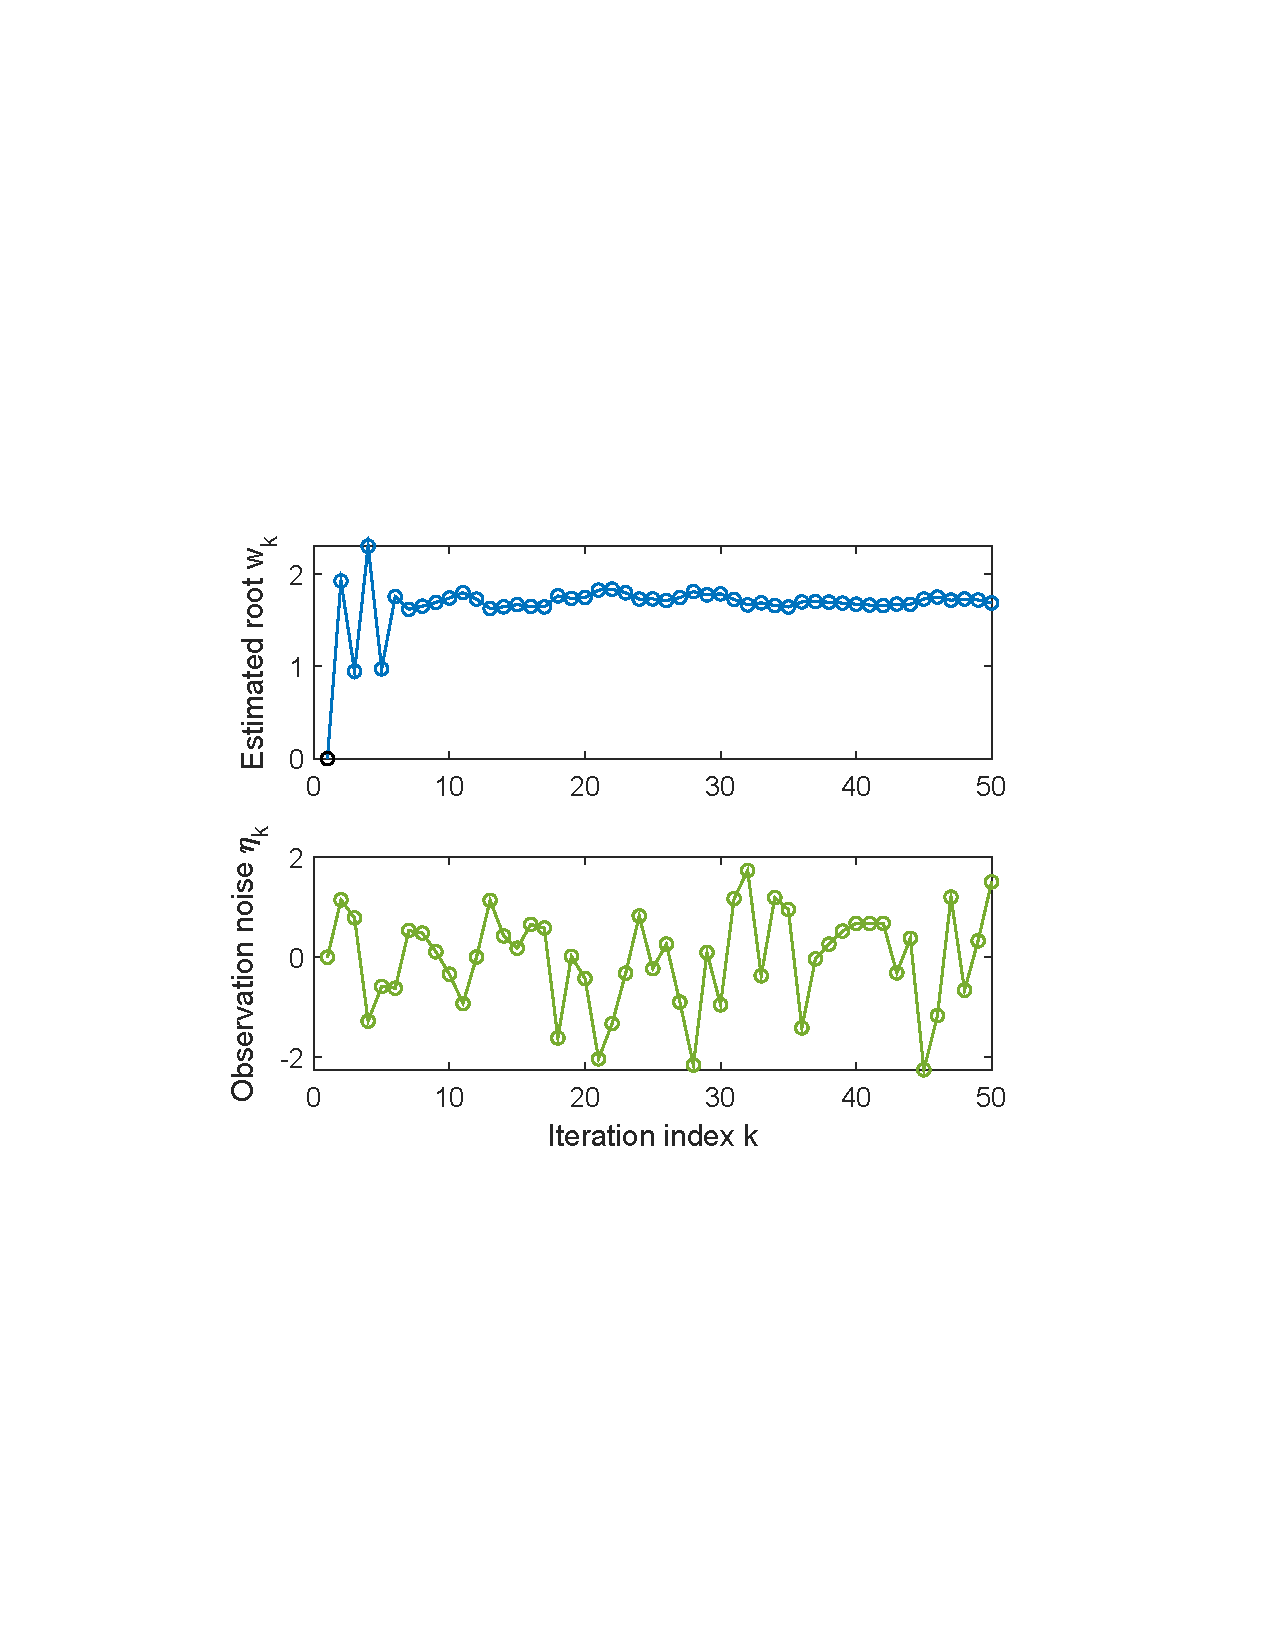
\includegraphics[width=0.4\linewidth]{chapterSA_fig_RMAlgoDemo}
%  \caption{An illustrative example of the RM algorithm.}
%  \label{chapterSA_fig_RMAlgoDemo}
%\end{figure}
%}
%\end{frame}
%---------------------
\subsection{Convergence analysis}
\begin{frame}
\frametitle{Outline}
\tableofcontents[currentsection]
\end{frame}
%-----------------------------
\begin{frame}
\frametitle{Robbins-Monro algorithm -- Convergence properties}

Why can the RM algorithm find the root of $g(w)=0$?

\begin{itemize}
\item First present an illustrative example.
\item Second give the rigorous convergence analysis.
\end{itemize}

\end{frame}
%-----------------------------
\begin{frame}
\frametitle{Robbins-Monro algorithm -- Convergence properties}

An illustrative example:
\begin{itemize}
\item $g(w)=\tanh(w-1)$
\item The true root of $g(w)=0$ is $w^*=1$.
\item Parameters: $w_1=3$, $a_k=1/k$, $\eta_k\equiv0$ (no noise for the sake of simplicity)
\end{itemize}

\pause
\vspace{10pt}
The RM algorithm in this case is $$\blue{w_{k+1}=w_k-a_kg(w_k)}$$
since $\tilde{g}(w_k,\eta_k)=g(w_k)$ when $\eta_k=0$.

\end{frame}
%---------------------
\begin{frame}
\frametitle{Robbins-Monro algorithm -- Convergence properties}
\vspace{-10pt}
Simulation result: $w_k$ converges to the true root $w^*=1$.
\begin{figure}
  \centering
  \includegraphics[width=0.5\linewidth]{chapterSA_fig_RMConvergenceDemo}
  %\caption{An example to illustrate the convergence of the RM algorithm.}
  %\label{chapterSA_fig_RMConvergenceDemo}
\end{figure}
\vspace{-10pt}
\pause
Intuition: \red{$w_{k+1}$ is closer to $w^*$ than $w_k$.}
\pause
\begin{itemize}
\item When \blue{$w_k>w^*$}, we have $g(w_k)>0$. Then, \blue{$w_{k+1}=w_k-a_kg(w_k)<w_k$} and hence $w_{k+1}$ is closer to $w^*$ than $w_k$.
\pause
\item When \blue{$w_k<w^*$}, we have $g(w_k)<0$. Then, \blue{$w_{k+1}=w_k-a_kg(w_k)>w_k$} and $w_{k+1}$ is closer to $w^*$ than $w_k$.
\end{itemize}
\end{frame}
%---------------------
\begin{frame}
\frametitle{Robbins-Monro algorithm -- Convergence properties}

The above analysis is intuitive, but not rigorous. A rigorous convergence result is given below.

\begin{theorem}[Robbins-Monro Theorem]\label{theorem_RMAlgo}
In the Robbins-Monro algorithm, if
\begin{enumerate}
\item $0<c_1\le\nabla_wg(w)\le c_2$ for all $w$;
\item $\sum_{k=1}^\infty a_k=\infty$ and $\sum_{k=1}^\infty a_k^2<\infty$;
\item $\E[\eta_k|\H_k]=0$ and $\E[\eta_k^2|\H_k]<\infty$;
\end{enumerate}
where $\H_k=\{w_k,w_{k-1},\dots\}$, then $w_k$ converges with probability 1 (w.p.1) to the root $w^*$ satisfying $g(w^*)=0$.
\end{theorem}

\end{frame}
%---------------------
\begin{frame}
\frametitle{Robbins-Monro algorithm -- Convergence properties}
Explanation of the three conditions:
\vspace{10pt}
\pause
\begin{itemize}
\item \textbf{Condition 1:} $0<c_1\le\nabla_wg(w)\le c_2$ for all $w$
{\small
\begin{itemize}
\item[-] $g$ should be \blue{monotonically increasing},which ensures that the root of $g(w)=0$ exists and is unique.
\item[-] The gradient is bounded from the above.
\item[-] This condition is not strict. Consider the example $g(w)=\nabla_w J(w)=0$. This condition requires that $J(w)$ is convex.
\end{itemize}}
\vspace{10pt}
\pause
\item \textbf{Condition 2:} $\sum_{k=1}^\infty a_k=\infty$ and $\sum_{k=1}^\infty a_k^2<\infty$
{\small
\begin{itemize}
\item[-] $\sum_{k=1}^\infty a_k^2<\infty$ ensures that \blue{$a_k$ converges to zero as $k\rightarrow\infty$}.
\item[-] $\sum_{k=1}^\infty a_k=\infty$ ensures that \blue{$a_k$ do not converge to zero too fast.}
\end{itemize}}
\vspace{10pt}
\pause
\item \textbf{Condition 3:} $\E[\eta_k|\H_k]=0$ and $\E[\eta_k^2|\H_k]<\infty$
{\small
\begin{itemize}
\item[-] A special yet common case is that $\{\eta_k\}$ is an iid stochastic sequence satisfying $\E[\eta_k]=0$ and $\E[\eta_k^2]<\infty$. The observation error $\eta_k$ is not required to be Gaussian.
\end{itemize}
}
\end{itemize}

\end{frame}
%---------------------
\begin{frame}
\frametitle{Robbins-Monro algorithm -- Convergence properties}
Examine \blue{Condition 2} more closely:
$$\sum_{k=1}^\infty a_k^2<\infty \qquad \sum_{k=1}^\infty a_k=\infty$$

\begin{itemize}
\item First, $\sum_{k=1}^\infty a_k^2<\infty$ indicates that $a_k\rightarrow0$ as $k\rightarrow\infty$.
\pause

\vspace{10pt}
\textbf{Why is this condition important?}

Since
$$w_{k+1}-w_k=-a_k\tilde{g}(w_k,\eta_k),$$
\begin{itemize}
\item[-] If $a_k\rightarrow0$, then $a_k\tilde{g}(w_k,\eta_k)\rightarrow0$ and hence \blue{$w_{k+1}-w_k\rightarrow0$}.

\item[-] We need the fact that $w_{k+1}-w_k\rightarrow0$ if $w_k$ converges eventually.

\item[-] If $w_k\rightarrow w^*$, $g(w_k)\rightarrow0$ and $\tilde{g}(w_k,\eta_k)$ is dominant by $\eta_k$.
\end{itemize}
\end{itemize}
\end{frame}
%---------------------
\begin{frame}
\frametitle{Robbins-Monro algorithm -- Convergence properties}
Examine \blue{Condition 2} more closely:
$$\sum_{k=1}^\infty a_k^2<\infty \qquad \sum_{k=1}^\infty a_k=\infty$$

\begin{itemize}
\item Second, $\sum_{k=1}^\infty a_k=\infty$ indicates that $a_k$ should not converge to zero too fast.

\vspace{10pt}
\pause
\textbf{Why is this condition important?}

{\small
Summarizing $w_{2}=w_1-a_1 \tilde{g}(w_1,\eta_1)$, $w_{3}=w_2-a_2 \tilde{g}(w_2,\eta_2)$, $\dots$, $w_{k+1}=w_k-a_k \tilde{g}(w_k,\eta_k)$ leads to
$$w_1-w_\infty=\sum_{k=1}^\infty a_k\tilde{g}(w_k,\eta_k).$$
Suppose $w_\infty=w^*$. If $\sum_{k=1}^\infty a_k<\infty$, then $\sum_{k=1}^\infty a_k\tilde{g}(w_k,\eta_k)$ may be bounded. Then, if the initial guess $w_1$ is chosen arbitrarily far away from $w^*$, then the above equality would be invalid.}
\end{itemize}
\end{frame}
%---------------------
\begin{frame}
\frametitle{Robbins-Monro algorithm -- Convergence properties}
\blue{What $\{a_k\}$ satisfies the two conditions? $\sum_{k=1}^\infty a_k^2<\infty, \sum_{k=1}^\infty a_k=\infty$}

\pause
One typical sequence is
\red{
$$a_k=\frac{1}{k}$$}
\vspace{-10pt}
\pause
\begin{itemize}
\item It satisfies \blue{$\sum_{k=1}^\infty a_k=\infty$} since
$$\lim_{n\rightarrow\infty} \left(\sum_{k=1}^n\frac{1}{k}-\ln n\right)=\kappa,$$
where $\kappa\approx0.577$ is called the Euler-Mascheroni constant (also called Euler's constant). %[See wiki].
\pause
\item It satisfies \blue{$\sum_{k=1}^\infty a_k^2<\infty$} since
$$\sum_{k=1}^\infty\frac{1}{k^2}=\frac{\pi^2}{6}<\infty.$$
The limit $\sum_{k=1}^\infty{1}/{k^2}$ also has a specific name in the number theory: Basel problem.
\end{itemize}
\end{frame}
%%---------------------
%\begin{frame}
%\frametitle{Robbins-Monro algorithm -- Convergence properties}
%If the three conditions are not satisfied, the algorithm may not work.
%\begin{itemize}
%\item For example, $g(w)=w^3-5$ does not satisfy the first condition on gradient boundedness. If the initial guess is good, the algorithm can converge (locally). Otherwise, it will diverge.
%\end{itemize}
%
%\pause
%We will see that $a_k$ is often selected as a \blue{sufficiently small constant} in many RL algorithms. Although the second condition is not satisfied in this case, the algorithm can still work effectively.
%
%\end{frame}
%---------------------
\subsection{Application to mean estimation}
\begin{frame}
\frametitle{Outline}
\tableofcontents[currentsection]
\end{frame}
%-----------------------------
\begin{frame}
\frametitle{Robbins-Monro algorithm -- Apply to mean estimation}

\blue{Recall} that
$$w_{k+1}=w_k+\alpha_k(x_k-w_k).$$
is the mean estimation algorithm introduced at the beginning of this lecture.

\pause
\begin{itemize}
\item If $\alpha_k=1/k$, then $w_{k+1}=1/k\sum_{i=1}^k x_i$.
\item If $\alpha_k$ is not $1/k$, the convergence was not analyzed.
\end{itemize}

\pause
Next, we show that this algorithm is \blue{a special case of the RM algorithm.}
Then, its convergence naturally follows.

\end{frame}
%---------------------
\begin{frame}
\frametitle{Robbins-Monro algorithm -- Apply to mean estimation}
{\small
1) Consider a function:
\begin{align*}
g(w)&\doteq w-\E[X].
\end{align*}
Our aim is to solve $g(w)=0$. If we can do that, then we can obtain $\E[X]$.
\begin{itemize}
\item[-] \blue{Mean estimation (i.e., finding $\E[X]$)} is formulated as a root-finding problem \blue{(i.e., solving $g(w)=0)$}.
\pause
\item[-] \textbf{Question:} Do we know the expression of $g(w)$ here?
\end{itemize}

\vspace{5pt}

\pause
2) The observation we can get is
\begin{align*}
\tilde{g}(w,x)&\doteq w-x,
\end{align*}
because we can only obtain samples of $X$.
Note that
\begin{align*}
\tilde{g}(w,\eta)
=w-x&=w-x+\E[X]-\E[X]\\
&=(w-\E[X])+(\E[X]-x)\doteq g(w)+\eta,
\end{align*}

\vspace{5pt}

\pause
3) The RM algorithm for solving $g(w)=0$ is
\begin{align*}
w_{k+1}=w_k-\alpha_k \tilde{g}(w_k,\eta_k)=w_k-\alpha_k(w_k-x_k),
\end{align*}
which is exactly the mean estimation algorithm.

The convergence naturally follows.
}
\end{frame}
%---------------------
\begin{frame}
\frametitle{Dvoretzky��s convergence theorem (optional)}
{\footnotesize
\begin{theorem}[Dvoretzky's Theorem]
Consider a stochastic process
$$w_{k+1}=(1-\alpha_k)w_k+\beta_k \eta_k,$$
where $\{\alpha_k\}_{k=1}^\infty,\{\beta_k\}_{k=1}^\infty,\{\eta_k\}_{k=1}^\infty$ are stochastic sequences. Here $\alpha_k\ge0,\beta_k\ge0$ for all $k$. Then, $w_k$ would converge to zero with probability 1 if the following conditions are satisfied:
\begin{enumerate}
\item $\sum_{k=1}^\infty \alpha_k=\infty$, $\sum_{k=1}^\infty \alpha_k^2<\infty$; $\sum_{k=1}^\infty \beta_k^2<\infty$ uniformly w.p.1;
\item $\E[\eta_k|\H_k]=0$ and $\E[\eta_k^2|\H_k]\le C$ w.p.1;
\end{enumerate}
where $\H_k=\{w_k,w_{k-1},\dots,\eta_{k-1},\dots,\alpha_{k-1},\dots,\beta_{k-1},\dots\}$.
%All the random variables are allowed to depend on the history $\H_k$.
\end{theorem}
}

\begin{itemize}
\item A more general result than the RM theorem.
\begin{itemize}
\item[-]It can be used to prove the RM theorem

\item[-] It can be used to analyze the mean estimation problem.

\item[-] An extension of it can be used to analyze Q-learning and TD learning algorithms.
\end{itemize}
\end{itemize}

\end{frame}
%--------------------------------------
\AtBeginSection[]% put it to the start of each section
{
  \begin{frame}
    \frametitle{Outline}
    \tableofcontents[currentsection]
  \end{frame}
}
\section{Stochastic gradient descent}
%---------------------
\subsection{Algorithm description}
\begin{frame}
\frametitle{Outline}
\tableofcontents[currentsection]
\end{frame}
%---------------------
\begin{frame}
\frametitle{Stochastic gradient descent}

Next, we introduce stochastic gradient descent (SGD) algorithms:
\begin{itemize}
\item SGD is widely used in the field of machine learning and also in RL.
\begin{itemize}
\item[-] SGD is a special RM algorithm.
\item[-] The mean estimation algorithm is a special SGD algorithm.
\end{itemize}
\end{itemize}

\pause
\vspace{15pt}
Problem setup: Suppose we aim to solve the following \blue{optimization problem}:
\begin{align*}%\label{eq_SGDOptimizationProblem}
\min_w\quad  J(w)=\E[f(w,X)]
\end{align*}
\begin{itemize}
\item $w$ is the parameter to be optimized.
\item $X$ is a random variable. The expectation is with respect to $X$.
\item $w$ and $X$ can be either scalars or vectors. The function $f(\cdot)$ is a scalar.
\end{itemize}
\end{frame}
%---------------------
\begin{frame}
\frametitle{Stochastic gradient descent}

\textbf{Method 1: gradient descent (GD)}
\begin{align*}%\label{chapterSA_eq_GDAlgo}
w_{k+1}=w_k-\alpha_k \blue{\nabla_w} \E[f(w_k,X)]\onslide<2->{=w_k-\alpha_k \E[\blue{\nabla_w} f(w_k,X)]}
\end{align*}
\pause\pause
\blue{Drawback:} Calculating the expectation requires the distribution of $X$.

\pause
\vspace{10pt}
\textbf{Method 2: batch gradient descent (BGD)}
$$\E[\nabla_w f(w_k,X)]\approx\frac{1}{n}\sum_{i=1}^n \nabla_w f(w_k,x_i)$$
Hence
\begin{align*}%\label{chapterSA_eq_BGDAlgo}
w_{k+1}=w_k-\alpha_k\frac{1}{n}\sum_{i=1}^n \nabla_w f(w_k,x_i)
\end{align*}
\pause
\blue{Drawback:} it requires many samples in each iteration for each $w_k$.

\end{frame}
%---------------------
\begin{frame}
\frametitle{Stochastic gradient descent -- Algorithm}

\textbf{Method 3: stochastic gradient descent (SGD)}
\begin{align*}%\label{chapterSA_eq_SGDAlgo}
w_{k+1}=w_k-\alpha_k \nabla_w f(w_k,x_k),
\end{align*}
\begin{itemize}
\item Compared to the gradient descent method:
\begin{itemize}
\item[-] Replace the \blue{true gradient $\E[\nabla_w f(w_k,X)]$} by the \blue{stochastic gradient $\nabla_w f(w_k,x_k)$}.
\end{itemize}
\item Compared to the batch gradient descent method:
\begin{itemize}
\item[-] let $n=1$.
\end{itemize}
\end{itemize}
\end{frame}
%---------------------
\subsection{Examples and application}
\begin{frame}
\frametitle{Outline}
\tableofcontents[currentsection]
\end{frame}
%---------------------
\begin{frame}
\frametitle{Stochastic gradient descent -- Example and application}
We next consider an example:
\begin{align*}%\label{eq_SGDMeanEst}
\min_w\quad  J(w)=\E[f(w,X)]=\E\left[\frac{1}{2}\|w-X\|^2\right],
\end{align*}
\pause
where
$$f(w,X)=\|w-X\|^2/2\qquad \nabla_wf(w,X)=w-X$$

\vspace{15pt}

\pause
\textbf{Exercises:}

\begin{itemize}
\item Exercise 1: Show that the optimal solution is $w^*=\E[X]$.

\item Exercise 2: Write out the GD algorithm for solving this problem.

\item Exercise 3: Write out the SGD algorithm for solving this problem.
\end{itemize}
\end{frame}
%---------------------
\begin{frame}
\frametitle{Stochastic gradient descent -- Example and application}
We next consider an example:
\begin{align*}%\label{eq_SGDMeanEst}
\min_w\quad  J(w)=\E[f(w,X)]=\E\left[\frac{1}{2}\|w-X\|^2\right],
\end{align*}

where
$$f(w,X)=\|w-X\|^2/2\qquad \nabla_wf(w,X)=w-X$$

\noindent\rule{11cm}{0.4pt}
\begin{itemize}
\item \textbf{Exercise 1:} Show that the optimal solution is $w^*=\E[X]$.
\item \textbf{Answer to exercise 1:} The optimal solution $w^*$ must satisfy
\begin{align*}
\nabla_w J(w)=0
\end{align*}
which is
\begin{align*}
\nabla_w \E\left[\frac{1}{2}\|w-X\|^2\right]
=\E\left[\nabla_w \frac{1}{2}\|w-X\|^2\right]
=\E\left[w-X\right]=0
\end{align*}
Therefore, we formulate the \blue{mean estimation problem (i.e., finding $\E[X]$)} as an \blue{optimization problem (i.e., optimizing $J(w)$)}.
\end{itemize}
\end{frame}
%---------------------
\begin{frame}
\frametitle{Stochastic gradient descent -- Example and application}
We next consider an example:
\begin{align*}%\label{eq_SGDMeanEst}
\min_w\quad  J(w)=\E[f(w,X)]=\E\left[\frac{1}{2}\|w-X\|^2\right],
\end{align*}

where
$$f(w,X)=\|w-X\|^2/2\qquad \nabla_wf(w,X)=w-X$$

\noindent\rule{11cm}{0.4pt}

\begin{itemize}
\item \textbf{Exercise 2:} Write out the GD algorithm for solving this problem.
\item \textbf{Answer to exercise 2:} The \blue{GD} algorithm for solving the above problem is
\begin{align*}
w_{k+1}
&=w_k-\alpha_k \nabla_w J(w_k)\\
&=w_k-\alpha_k \E[\nabla_w f(w_k,X)]\\
&=w_k-\alpha_k \E[w_k-X].
\end{align*}
\end{itemize}
\end{frame}
%---------------------
\begin{frame}
\frametitle{Stochastic gradient descent -- Example and application}
We next consider an example:
\begin{align*}%\label{eq_SGDMeanEst}
\min_w\quad  J(w)=\E[f(w,X)]=\E\left[\frac{1}{2}\|w-X\|^2\right],
\end{align*}

where
$$f(w,X)=\|w-X\|^2/2\qquad \nabla_wf(w,X)=w-X$$

\noindent\rule{11cm}{0.4pt}

\begin{itemize}
\item \textbf{Exercise 3:} Write out the SGD algorithm for solving this problem.
\item \textbf{Answer to exercise 3:}
The \blue{SGD} algorithm for solving the above problem is
$$w_{k+1}
=w_k-\alpha_k \nabla_w f(w_k,x_k)
=w_k-\alpha_k (w_k-x_k)$$

\begin{itemize}
\item[-] It is the same as the mean estimation algorithm we presented before.
\item[-] Therefore, that mean estimation algorithm is a special SGD algorithm.
\end{itemize}
\end{itemize}
\end{frame}
%---------------------
\subsection{Convergence analysis}
\begin{frame}
\frametitle{Outline}
\tableofcontents[currentsection]
\end{frame}
%---------------------
\begin{frame}
\frametitle{Stochastic gradient descent -- Convergence}
\textbf{Idea of SGD:}
\vspace{-10pt}
\begin{align*}
w_{k+1}=w_k-&\alpha_k \E[\nabla_w f(w_k,X)]\\
&\Downarrow\\
w_{k+1}=w_k-&\alpha_k \nabla_w f(w_k,x_k)
\end{align*}
where the \blue{true gradient} $\E[\nabla_w f(w_k,X)]$ is replaced by the \blue{stochastic gradient} $\nabla_w f(w_k,X)$.

\vspace{5pt}
\pause
\textbf{Question:} Since $$\nabla_w f(w_k,x_k)\ne \E[\nabla_w f(w,X)]$$
\blue{whether $w_k\rightarrow w^*$ as $k\rightarrow\infty$ by SGD?}

\vspace{5pt}
\pause
\textbf{Observation:} The stochastic gradient is a noisy measurement of the true gradient:
\begin{align*}
\nabla_w f(w_k,x_k)=\E[\nabla_w f(w,X)]+\underbrace{\nabla_w f(w_k,x_k)-\E[\nabla_w f(w,X)]}_{\eta}
\end{align*}
where $\eta$ is the noise.
\end{frame}
%---------------------
\begin{frame}
\frametitle{Stochastic gradient descent -- Convergence}

We next show that \blue{SGD is a special RM algorithm}. Then, the convergence naturally follows.

\pause
\vspace{10pt}
\blue{The aim of SGD} is to minimize
$$J(w)=\E[f(w,X)]$$
\pause
This problem can be converted to a \blue{root-finding} problem:
$$\nabla_w J(w)=\E[\nabla_w f(w,X)]=0$$
\pause
Let
$$g(w)=\nabla_w J(w)=\E[\nabla_w f(w,X)]$$
Then, \red{the aim of SGD is to find the root of $g(w)=0$}.

\end{frame}
%---------------------
\begin{frame}
\frametitle{Stochastic gradient descent -- Convergence}

What we can measure is
\begin{align*}
\tilde{g}(w,\eta)
&=\nabla_w f(w,x)\\
&=\underbrace{\E[\nabla_w f(w,X)]}_{g(w)}+\underbrace{\nabla_w f(w,x)-\E[\nabla_w f(w,X)]}_{\eta}.
\end{align*}

\pause
Then, the RM algorithm for solving $g(w)=0$ is
\begin{align*}
w_{k+1}=w_k-a_k \tilde{g}(w_k,\eta_k)=w_k-a_k\nabla_w f(w_k,x_k).
\end{align*}
\begin{itemize}
\item \red{It is exactly the SGD algorithm.}

\item Therefore, SGD is a special RM algorithm.
\end{itemize}
\end{frame}
%---------------------
\begin{frame}
\frametitle{Stochastic gradient descent -- Convergence}

Since SGD is a special RM algorithm, its convergence naturally follows.

\begin{theorem}[Convergence of SGD]\label{theorem_SGDConvergence}
In the SGD algorithm, if
\begin{enumerate}
\item $0<c_1\le\nabla_w^2 f(w,X)\le c_2$;
\item $\sum_{k=1}^\infty a_k=\infty$ and $\sum_{k=1}^\infty a_k^2<\infty$;
\item $\{x_k\}_{k=1}^\infty$ is iid;
\end{enumerate}
then $w_k$ converges to the root of $\nabla_w\E[f(w,X)]=0$ with probability 1.
\end{theorem}

For the proof see the book.

\end{frame}

%---------------------
\subsection{Convergence pattern}
\begin{frame}
\frametitle{Outline}
\tableofcontents[currentsection]
\end{frame}
%---------------------
\begin{frame}
\frametitle{Stochastic gradient descent -- Convergence pattern}
\textbf{Idea of SGD:}
\vspace{-10pt}
\begin{align*}
w_{k+1}=w_k-&\alpha_k \E[\nabla_w f(w_k,X)]\\
&\Downarrow\\
w_{k+1}=w_k-&\alpha_k \nabla_w f(w_k,x_k)
\end{align*}
where the \blue{true gradient} $\E[\nabla_w f(w_k,X)]$ is replaced by the \blue{stochastic gradient} $\nabla_w f(w_k,X)$.

\vspace{10pt}
\textbf{Question: }
Since the stochastic gradient is random, \blue{whether the convergence of SGD is slow or random?}

\end{frame}
%---------------------
\begin{frame}
\frametitle{Stochastic gradient descent -- Convergence pattern}

\textbf{Example:} {\small$X\in\R^2$ represents a random position in the plane. Its distribution is uniform in the square area centered at the origin with the side length as 20. The true mean is $\E[X]=0$. The mean estimation is based on 100 iid samples $\{x_i\}_{i=1}^{100}$.}

\begin{figure}
  \centering
  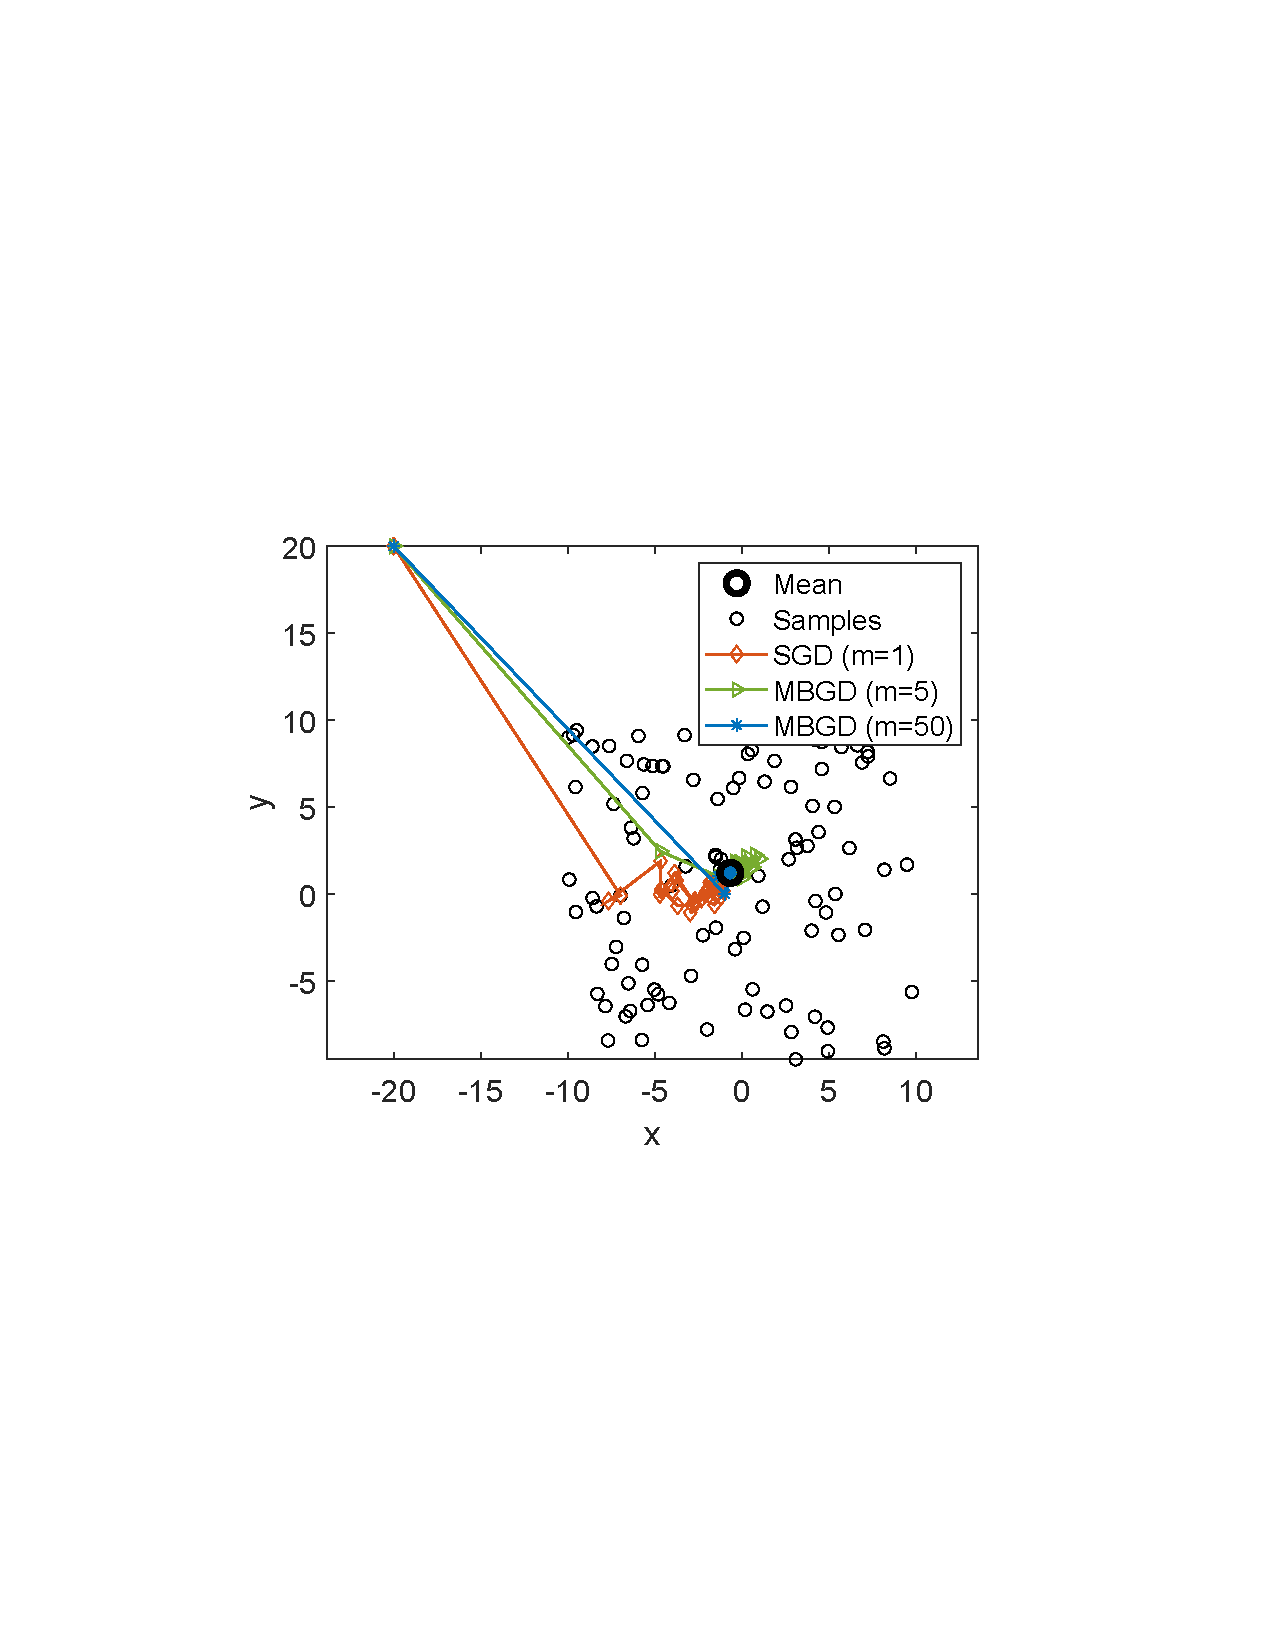
\includegraphics[width=0.45\linewidth]{fig_meanEstTraj}
  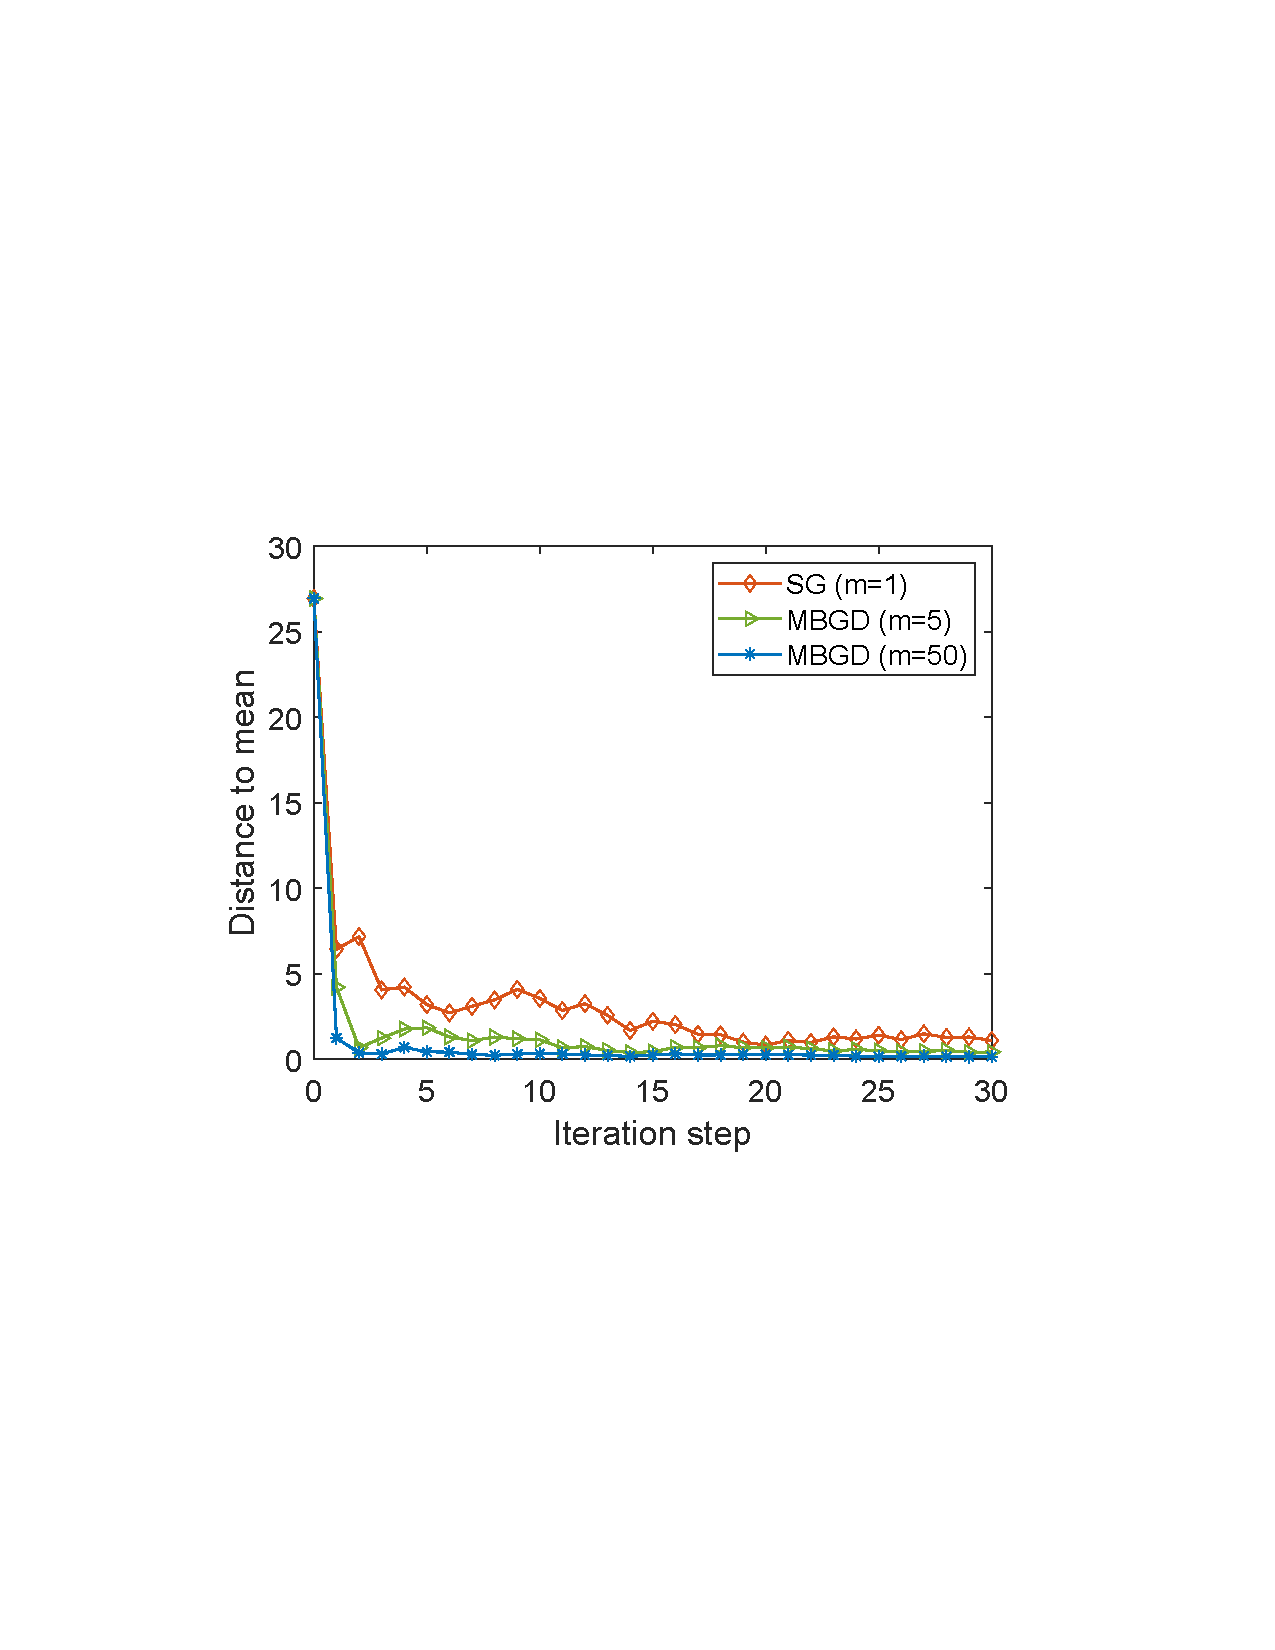
\includegraphics[width=0.45\linewidth]{fig_meanEstErr}
\end{figure}
\pause
Observations:
\begin{itemize}
\item When the estimate (e.g., the initial guess) is \blue{far away} from the true value, the SGD estimate can approach the neighborhood of the true value fast.
\item When the estimate is \blue{close to} the true value, it exhibits certain randomness but still approaches the true value gradually.
\end{itemize}

\end{frame}
%---------------------
\begin{frame}
\frametitle{Stochastic gradient descent -- Convergence pattern}
\textbf{Question:} Why such a pattern?

\textbf{Answer:} We answer this question by considering the \red{relative error} between the stochastic and batch gradients:
\begin{align*}
\delta_{k}\doteq\frac{|\nabla_w f(w_k,x_k)-\E[\nabla_w f(w_k,X)]|}{|\E[\nabla_w f(w_k,X)]|}.
\end{align*}
\pause
It can be proven that
\begin{align*}
\delta_{k}
\le \frac{\big|\nabla_w f(w_k,x_k)-\E[\nabla_w f(w_k,X)]\big|}{c|w_k-w^*|}.
\end{align*}
The proof is given in the next slide. The proof is optional.
\end{frame}
%---------------------
\begin{frame}
\frametitle{Stochastic gradient descent -- Convergence pattern (optional)}

Since $\E[\nabla_w f(w^*,X)]=0$, we have
{\small
\begin{align*}%\label{chapterSA_eq_relativeGradentError}
\delta_{k}
=\frac{|\nabla_w f(w_k,x_k)-\E[\nabla_w f(w_k,X)]|}{|\E[\nabla_w f(w_k,X)]-\E[\nabla_w f(w^*,X)]|}
=\frac{|\nabla_w f(w_k,x_k)-\E[\nabla_w f(w_k,X)]|}{|\E[\nabla^2_w f(\tilde{w}_k,X) (w_k-w^*)]|}
\end{align*}
}
where the last equality is due to the mean value theorem and $\tilde{w}_k\in[w_k,w^*]$.

Suppose $f$ is strictly convex such that
$$\nabla^2_w f\ge c>0$$
for all $w,X$, where $c$ is a positive bound.


Then, the denominator of $\delta_k$ becomes
\begin{align*}
\big|\E[\nabla^2_w f(\tilde{w}_k,X) (w_k-w^*)]\big|
&=\big|\E[\nabla^2_w f(\tilde{w}_k,X)](w_k-w^*)\big|\\
&=\big|\E[\nabla^2_w f(\tilde{w}_k,X)]\big|\big|(w_k-w^*)\big|
\ge c|w_k-w^*|.
\end{align*}

Substituting the above inequality to $\delta_k$ gives
\begin{align*}
\delta_{k}
\le \frac{\big|\nabla_w f(w_k,x_k)-\E[\nabla_w f(w_k,X)]\big|}{c|w_k-w^*|}.
\end{align*}
\end{frame}
%---------------------
\begin{frame}
\frametitle{Stochastic gradient descent -- Convergence pattern}

Note that
\begin{align*}
\delta_{k}
\le \frac{\big|\overbrace{\nabla_w f(w_k,x_k)}^{\text{stochastic gradient}}-\overbrace{\E[\nabla_w f(w_k,X)]}^{\text{true gradient}}\big|}{\underbrace{c|w_k-w^*|}_{\text{distance to the optimal solution}}}.
\end{align*}
\pause
The above equation suggests an interesting convergence pattern of SGD.
\begin{itemize}
\item The upper bound is inversely proportional to $|w_k-w^*|$.
\begin{itemize}
\item[-] \blue{When $|w_k-w^*|$ is large}, the relative error $\delta_k$ is small and \red{SGD behaves like GD}.
\item[-] \blue{When $|w_k-w^*|$ is small}, the relative error $\delta_k$ may be large (the upper bound may not be tight). Then, \red{SGD exhibits more randomness} in the neighborhood of $w^*$.
\end{itemize}
\end{itemize}
\end{frame}

%
%%---------------------
%\subsection{A deterministic formulation}
%\begin{frame}
%\frametitle{Outline}
%\tableofcontents[currentsection]
%\end{frame}
%%---------------------
%\begin{frame}
%\frametitle{Stochastic gradient descent -- A deterministic formulation}
%\begin{itemize}
%\item The formulation of SGD we introduced above involves random variables and expectation.
%
%\item One may often encounter a \blue{deterministic} formulation of SGD without involving any random variables.
%\end{itemize}
%
%\pause
%Consider the optimization problem:
%$$\min_w\quad  J(w)=\frac{1}{n}\sum_{i=1}^n f(w,x_i),$$
%\begin{itemize}
%\item $f(w,x_i)$ is a parameterized function.
%\item $w$ is the parameter to be optimized.
%\item a set of real numbers $\{x_i\}_{i=1}^n$, where $x_i$ does not have to be a sample of any random variable.
%\end{itemize}
%\end{frame}
%%---------------------
%\begin{frame}
%\frametitle{Stochastic gradient descent -- A deterministic formulation}
%The gradient descent algorithm for solving this problem is
%\begin{align*}%\label{eq_SGDAnotherStory}
%w_{k+1}=w_k-\alpha_k \nabla_w J(w_k)=w_k-\alpha_k \frac{1}{n}\sum_{i=1}^n \nabla_wf(w_k,x_{i}).
%\end{align*}
%\pause
%Suppose the set is large and we can only fetch a single number every time. In this case, we can use the following iterative algorithm:
%\begin{align*}%\label{chapterSA_eq_SGDAlgoDeterministic}
%w_{k+1}=w_k-\alpha_k \nabla_w f(w_k,x_{k}).
%\end{align*}
%
%\pause
%\textbf{Questions:}
%\begin{itemize}
%\item Is this algorithm SGD? It does not involve any random variables or expected values.
%\item How should we use the finite set of numbers $\{x_i\}_{i=1}^n$? Should we sort these numbers in a certain order and then use them one by one? Or should we randomly sample a number from the set?
%\end{itemize}
%\end{frame}
%%---------------------
%\begin{frame}
%\frametitle{Stochastic gradient descent -- A deterministic formulation}
%A quick answer to the above questions is that we can introduce a random variable manually and convert the \emph{deterministic formulation} to the \emph{stochastic formulation} of SGD.
%
%\pause
%In particular, suppose $X$ is a random variable defined on the set $\{x_i\}_{i=1}^n$. Suppose its probability distribution is uniform such that
%$$p(X=x_i)=1/n$$
%\pause
%Then, the deterministic optimization problem becomes a stochastic one:
%$$\min_w\quad  J(w)=\frac{1}{n}\sum_{i=1}^n f(w,x_i)=\E[f(w,X)].$$
%\vspace{-10pt}
%\pause
%{\small
%\begin{itemize}
%\item The last equality in the above equation is strict instead of approximate.
%Therefore, the algorithm is SGD.
%\item The estimate converges if $x_k$ is \emph{uniformly} and independently sampled from $\{x_i\}_{i=1}^n$. $x_k$ may repeatedly take the same number in $\{x_i\}_{i=1}^n$ since it is sampled randomly.
%\end{itemize}
%}
%\end{frame}
%---------------------
\subsection{BGD, MBGD, and SGD}
\begin{frame}
\frametitle{Outline}
\tableofcontents[currentsection]
\end{frame}
%---------------------
\begin{frame}
\frametitle{BGD, MBGD, and SGD}
Suppose we would like to minimize $J(w)=\E[f(w,X)]$ given a set of random samples $\{x_i\}_{i=1}^n$ of $X$.

\vspace{10pt}
The BGD, SGD, MBGD algorithms solving this problem are, respectively,
\begin{align*}
w_{k+1}&=w_k-\alpha_k \frac{1}{n}\sum_{i=1}^n \nabla_wf(w_k,x_{i}),\qquad \text{(BGD)}\\
w_{k+1}&=w_k-\alpha_k \frac{1}{m}\sum_{j\in\I_k} \nabla_wf(w_k,x_{j}),\qquad \text{(MBGD)}\\
w_{k+1}&=w_k-\alpha_k \nabla_w f(w_k,{x}_{k}).\qquad\qquad \text{(SGD)}
\end{align*}
\vspace{-10pt}
\pause
\begin{itemize}
{\small
\item \textbf{In the BGD algorithm}, all the samples are used in every iteration. When $n$ is large, $(1/n)\sum_{i=1}^n \nabla_wf(w_k,x_{i})$ is close to the true gradient $\E[\nabla_wf(w_k,X)]$.
\pause
\item \textbf{In the MBGD algorithm}, $\I_k$ is a subset of $\{1,\dots,n\}$ with the size as $|\I_k|=m$. The set $\I_k$ is obtained by $m$ times iid samplings.
\pause
\item \textbf{In the SGD algorithm}, $x_k$ is randomly sampled from $\{x_i\}_{i=1}^n$ at time $k$.
}
\end{itemize}
\end{frame}
%---------------------
\begin{frame}
\frametitle{BGD, MBGD, and SGD}
Compare MBGD with BGD and SGD:
\begin{itemize}
\item Compared to SGD, MBGD has less randomness because it uses more samples instead of just one as in SGD.
\pause
\item Compared to BGD, MBGD does not require to use all the samples in every iteration, making it more flexible and efficient.
\vspace{10pt}
\pause
\item If $m=1$, MBGD becomes SGD.
\pause
\item If $m=n$, MBGD does NOT become BGD strictly speaking because MBGD uses randomly fetched $n$ samples whereas BGD uses all $n$ numbers. In particular, MBGD may use a value in $\{x_i\}_{i=1}^n$ multiple times whereas BGD uses each number once.
\end{itemize}
\end{frame}
%---------------------
\begin{frame}
\frametitle{BGD, MBGD, and SGD -- Illustrative examples}
Given some numbers $\{x_i\}_{i=1}^n$, our aim is to calculate the mean $\bar{x}=\sum_{i=1}^n x_i/n$. This problem can be equivalently stated as the following optimization problem:
$$\min_w\quad  J(w)=\frac{1}{2n}\sum_{i=1}^n \|w-x_i\|^2$$

\pause
The three algorithms for solving this problem are, respectively,
{
\begin{align*}
w_{k+1}&=w_k-\alpha_k \frac{1}{n}\sum_{i=1}^n(w_k-x_i)=w_k-\alpha_k (w_k-\bar{x}), \qquad \text{(BGD)}\\
w_{k+1}&=w_k-\alpha_k \frac{1}{m}\sum_{j\in\I_k} (w_k-x_j)=w_k-\alpha_k \left(w_k-\bar{x}_{k}^{(m)}\right),\qquad \text{(MBGD)}\\
w_{k+1}&=w_k-\alpha_k (w_k-x_k), \qquad \text{(SGD)}
\end{align*}
}
where $\bar{x}_{k}^{(m)}=\sum_{j\in\I_k} x_j/m$.

\end{frame}
%%---------------------
%\begin{frame}
%\frametitle{BGD, MBGD, and SGD}
%
%Furthermore, if \blue{$\alpha_k=1/k$}, the above equation can be solved as
%\begin{align*}
%w_{k+1}&=\frac{1}{k}\sum_{j=1}^k \bar{x}=\bar{x},\qquad \text{(BGD)}\\
%w_{k+1}&=\frac{1}{k}\sum_{j=1}^k \bar{x}_{j}^{(m)},\qquad \text{(MBGD)}\\
%w_{k+1}&=\frac{1}{k}\sum_{j=1}^k x_j.\qquad \text{(SGD)}
%\end{align*}
%\begin{itemize}
%\item The estimate of BGD at each step is exactly the optimal solution $w^*=\bar{x}$.
%\item The estimate of MBGD approaches the mean faster than SGD because $\bar{x}_{k}^{(m)}$ is already an average.
%\end{itemize}
%\end{frame}
%---------------------
\begin{frame}
\frametitle{BGD, MBGD, and SGD}

Let $\alpha_k=1/k$. Given 100 points, using different mini-batch sizes leads to different convergence speed.

\begin{figure}
  \centering
  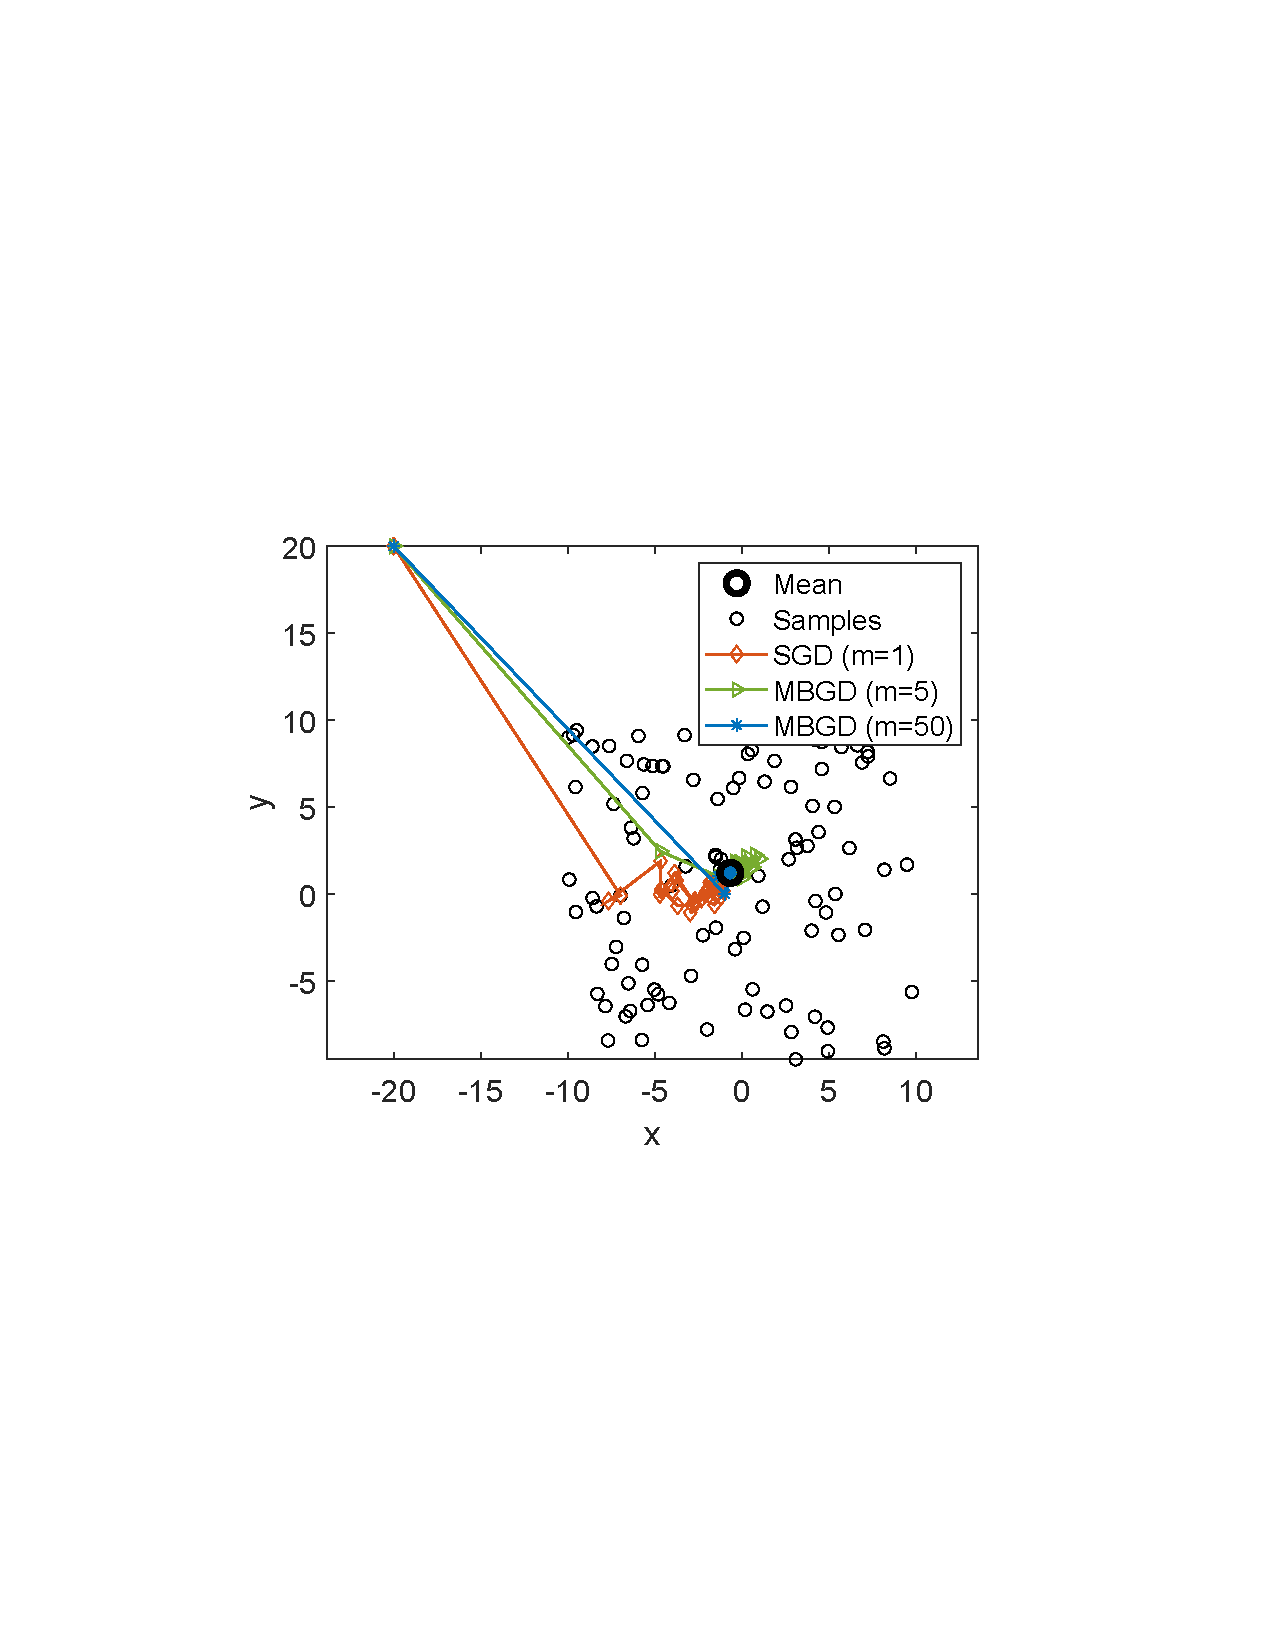
\includegraphics[width=0.5\linewidth]{fig_meanEstTraj}
  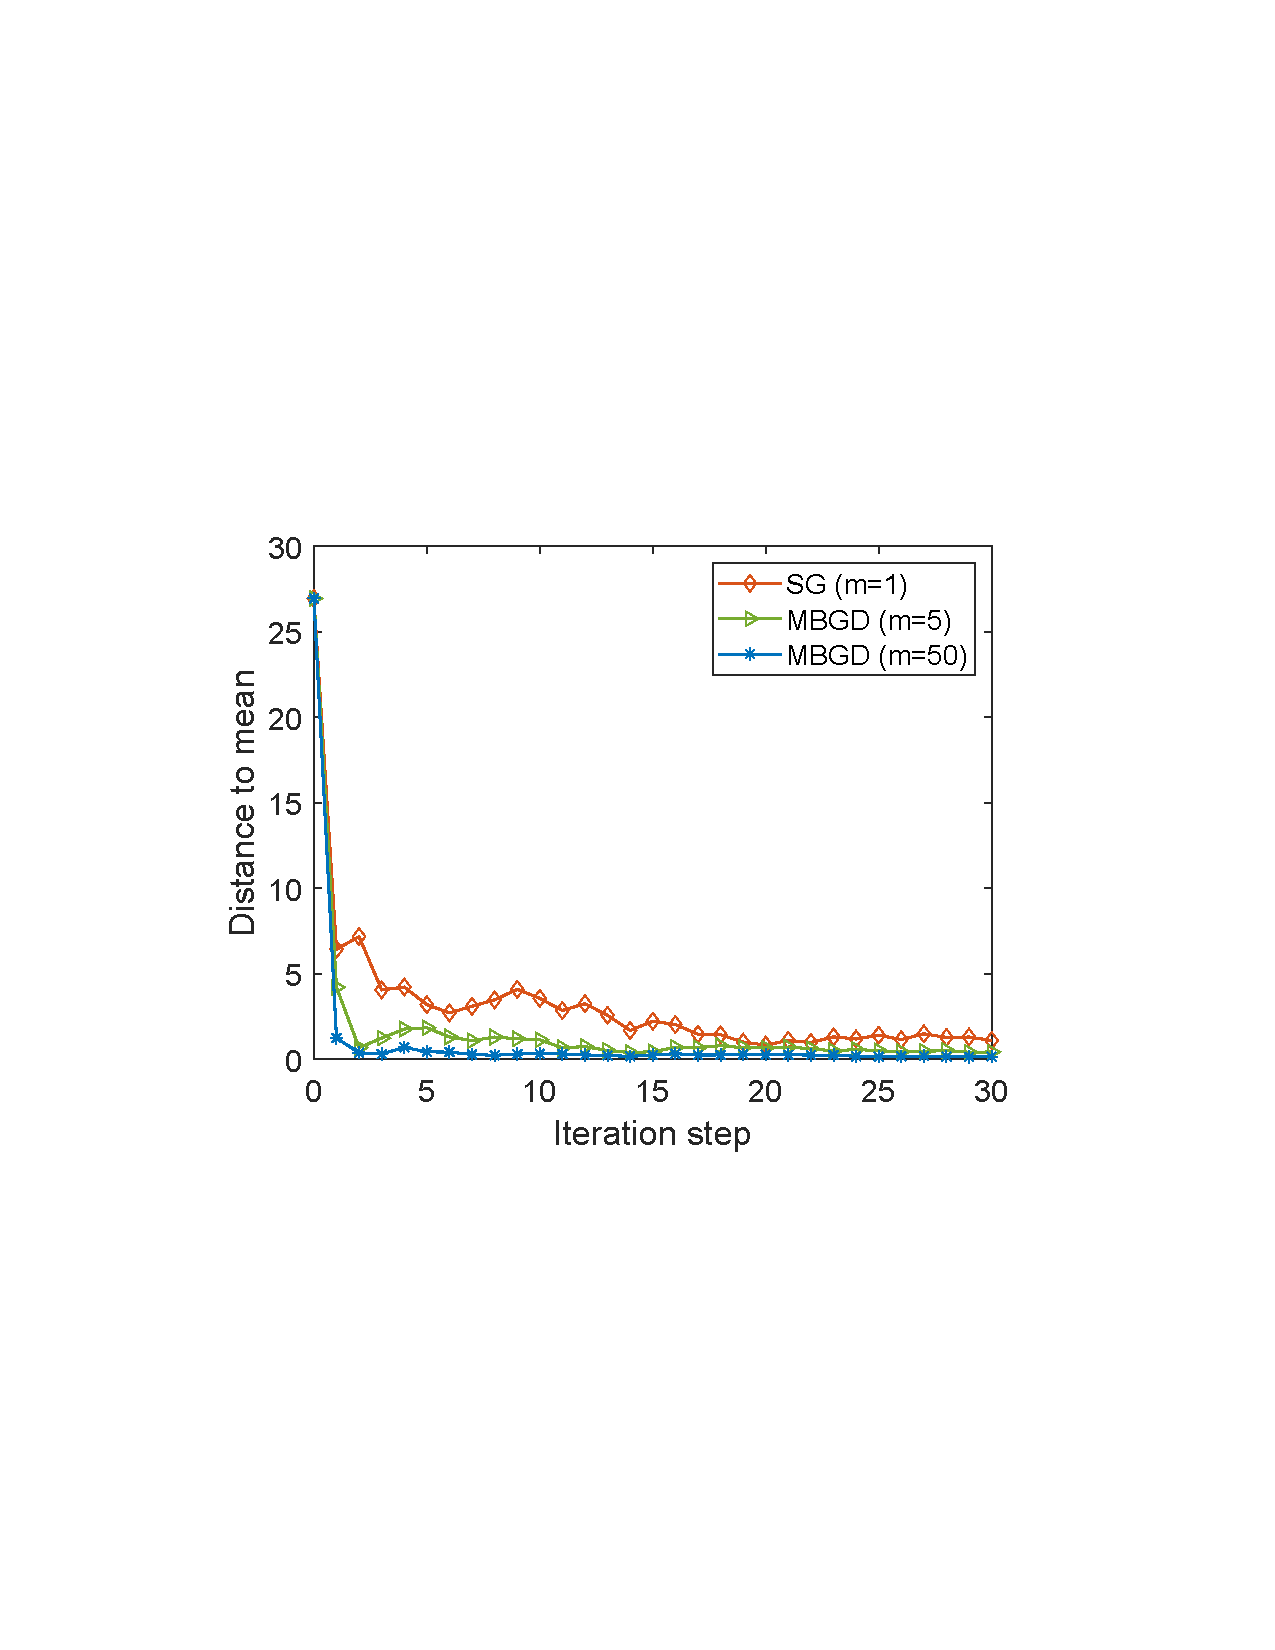
\includegraphics[width=0.5\linewidth]{fig_meanEstErr}
  \caption{An illustrative example for mean estimation by different GD algorithms.}
  \label{fig_meanEstDifferentGD}
\end{figure}

\end{frame}
%--------------------------------------
\AtBeginSection[]% put it to the start of each section
{
  \begin{frame}
    \frametitle{Outline}
    \tableofcontents[currentsection]
  \end{frame}
}
\section{Summary}
%---------------------
\begin{frame}
\frametitle{Summary}

\begin{itemize}
\item Mean estimation: compute $\E[X]$ using $\{x_k\}$
\begin{align*}%\label{eq_meanEstAlgok}
w_{k+1}=w_k-\frac{1}{k}(w_k-x_k).
\end{align*}
\item RM algorithm: solve $g(w)=0$ using $\{\tilde{g}(w_k,\eta_k)\}$
\begin{align*}%\label{chapterSA_RMAlgo}
w_{k+1}=w_k-a_k \tilde{g}(w_k,\eta_k)
\end{align*}
\item SGD algorithm: minimize $J(w)=\E[f(w,X)]$ using $\{\nabla_w f(w_k,x_k)\}$
\begin{align*}%\label{chapterSA_eq_SGDAlgo}
w_{k+1}=w_k-\alpha_k \nabla_w f(w_k,x_k),
\end{align*}
\end{itemize}

These results are useful:
\begin{itemize}
\item We will see in the next chapter that the temporal-difference learning algorithms can be viewed as stochastic approximation algorithms and hence have similar expressions.
\item They are important optimization techniques that can be applied to many other fields.
\end{itemize}

\end{frame}
%---------------------
%%%%%%%%%%%%%%%%%%%%%%%%%%%%%%%%%%%%%%%%%%%%%%%%%%%%%%%%%%%%%%%%%%%%%%%%%%%%%%%%%%%%%%%%%%%%%%%%%%
%\bibliographystyle{plainnat}
%\bibliography{myOwnPub,zsyReferenceAll}
\end{document}
